\chapter{Électronique~: rétroaction, oscillateurs et acquisition du signal}\label{ch:b2:feedback-oscillators}

Approchez trop un microphone du haut-parleur qu'il alimente et la salle
s'emplit d'un hurlement~: l'amplificateur s'entend lui-même, et un bruit minuscule croît
jusqu'au cri, sur une hauteur bien précise. Domestiquée, cette même boucle est le
cœur de toute horloge, de toute radio et de tout synthétiseur --- un \emph{oscillateur}
qui fabrique une sinusoïde à partir d'un simple gain et d'un filtre. Le volume de
première année construisait amplificateurs, filtres et comparateurs avec l'amplificateur
opérationnel~; ce chapitre referme la boucle autour d'eux, demande quand une
boucle est stable et quand elle oscille, construit deux oscillateurs --- l'un
sinusoïdal, l'autre carré --- puis passe aux deux opérations par
lesquelles un signal mesuré parvient à un ordinateur~: l'\emph{échantillonnage} et
l'extraction hors du bruit par \emph{\omterm{prop:b2:feedback-oscillators:lockin}{détection synchrone}}.

\begin{omfigure}
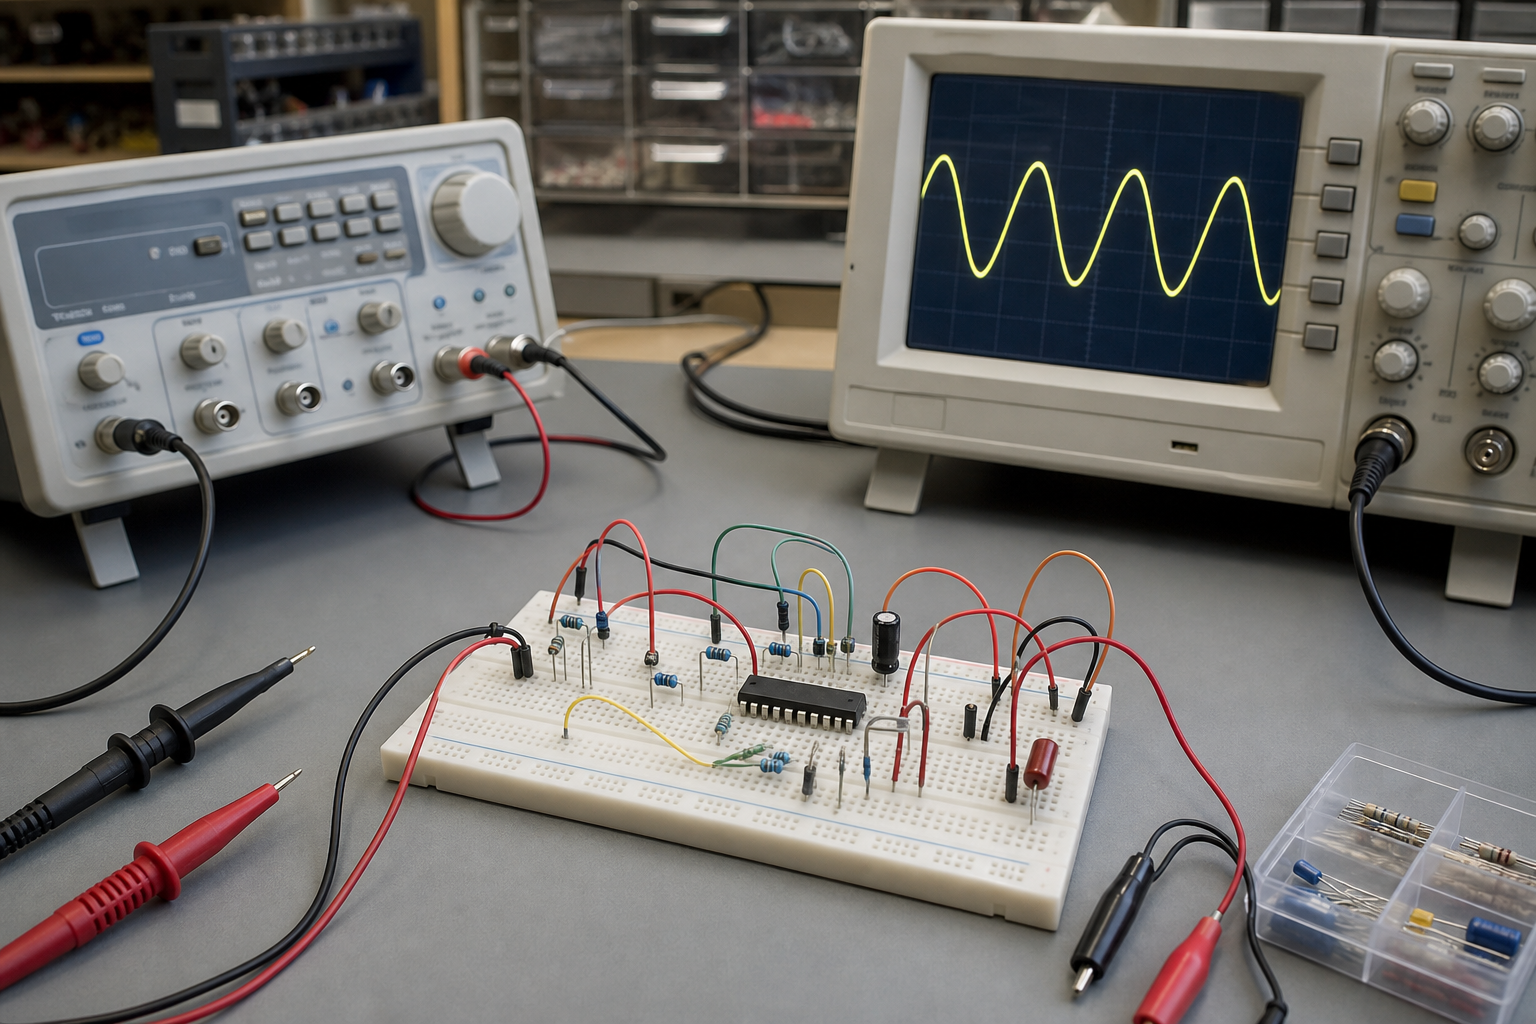
\includegraphics[width=0.58\linewidth]{images/book4/ai/b4-09-electronics-bench-oscillator.png}

{\small Une plaque d'essai, un générateur de fonctions et un oscilloscope~: la paillasse sur laquelle on referme une boucle de \omterm{def:b2:feedback-oscillators:loop}{rétroaction} --- et sur laquelle on découvre, lorsque l'amplificateur se met à chanter, qu'il est devenu un oscillateur.}
\end{omfigure}


\section{Rétroaction et stabilité}

\begin{definition}[Boucle fermée~; gain de boucle]\label{def:b2:feedback-oscillators:loop}
\index{rétroaction}\index{gain de boucle}\index{fonction de transfert en boucle fermée}
Un amplificateur de fonction de transfert $\underline A(\jmath\omega)$ reçoit
l'entrée $\underline e$ augmentée d'une fraction $\underline\beta(\jmath\omega)\,\underline s$ de sa propre
sortie $\underline s$ (rétroaction positive~; pour une rétroaction négative, changer le
signe de $\beta$). La fonction de transfert en \emph{boucle fermée} et le
\emph{gain de boucle} valent
\[
\underline H = \frac{\underline s}{\underline e} = \frac{\underline A}{1 - \underline A\,\underline\beta} ,
\qquad \underline T = \underline A\,\underline\beta .
\]
\end{definition}

\begin{theorem}[Stabilité d'une boucle linéaire~; condition d'oscillation]\label{thm:b2:feedback-oscillators:stability}
\index{stabilité (système linéaire)}\index{condition de Barkhausen}\index{équation caractéristique}
En remplaçant $\jmath\omega$ par la variable complexe $p$, l'évolution libre de
la boucle est gouvernée par les racines de son \emph{\omterm{thm:b2:feedback-oscillators:stability}{équation caractéristique}}
$1 - \underline A(p)\underline\beta(p) = 0$ (les pôles de $\underline H$)~: chaque racine
$p_i$ apporte un mode $\eu^{p_it}$. La boucle est \emph{stable} lorsque toutes les
racines sont de partie réelle négative (tout mode s'éteint)~; elle
\emph{oscille}, en amplitude croissante, lorsqu'une racine a une partie réelle
positive. La frontière --- une paire de racines imaginaires pures $\pm\jmath
\omega_0$, c'est-à-dire une sinusoïde entretenue --- est atteinte lorsque
\[
\underline A(\jmath\omega_0)\,\underline\beta(\jmath\omega_0) = 1
\]
(\emph{\omterm{thm:b2:feedback-oscillators:stability}{condition de Barkhausen}}~: \omterm{def:b2:feedback-oscillators:loop}{gain de boucle} de module un et de phase
nulle à $\omega_0$). Pour un dénominateur du second degré $ap^2 + bp + c$ la
boucle est stable si et seulement si $a$, $b$, $c$ sont de même signe.
\end{theorem}

\begin{proof}
L'équation différentielle de la boucle s'obtient à partir de $\underline s(1 -
\underline A\underline\beta) = \underline A\underline e$ en lisant chaque puissance de $\jmath\omega$
comme une dérivée temporelle~; ses solutions homogènes sont les $\eu^{p_it}$
où les $p_i$ sont les racines du polynôme. La croissance ou la décroissance suit le
signe de $\operatorname{Re}p_i$~; pour un polynôme du second degré les racines
sont de partie réelle négative exactement lorsque les coefficients sont de même signe
(leur somme vaut $-b/a$ et leur produit $c/a$). La \omterm{thm:b2:feedback-oscillators:stability}{condition de Barkhausen}
exprime l'existence d'une racine en $p = \jmath\omega_0$.
\end{proof}

\begin{remark}[Comment un oscillateur démarre et s'arrête]\label{rem:b2:feedback-oscillators:start}
Un oscillateur se conçoit avec un \omterm{def:b2:feedback-oscillators:loop}{gain de boucle} légèrement \emph{supérieur} à
un en $\omega_0$~: le bruit présent à la mise sous tension contient cette fréquence,
qui croît exponentiellement tandis que toutes les autres s'éteignent. La théorie linéaire
prévoit alors une amplitude infinie~; en réalité une \emph{non-linéarité} ---
la saturation de l'amplificateur, ou un élément volontairement non linéaire
--- abaisse le gain effectif à mesure que l'amplitude croît, jusqu'à ce que le
\omterm{def:b2:feedback-oscillators:loop}{gain de boucle} vaille en moyenne exactement un~: l'amplitude se stabilise. Tout oscillateur
réel est ainsi une boucle linéaire pour la fréquence et non linéaire
pour l'amplitude~; plus la limitation est douce, plus la sinusoïde est
pure.
\end{remark}

\section{L'oscillateur à pont de Wien}

\begin{proposition}[Oscillateur à pont de Wien]\label{prop:b2:feedback-oscillators:wien}
\index{oscillateur à pont de Wien}\index{réseau de Wien}
Un amplificateur opérationnel monté en non-inverseur de gain $K = 1 + R_2/R_1$
ramène sa sortie sur son entrée $+$ à travers le \emph{\omterm{prop:b2:feedback-oscillators:wien}{réseau de Wien}}~:
$R$ et $C$ en série, puis $R$ et $C$ en parallèle vers la masse. La
fonction de transfert du réseau vaut
\[
\underline\beta(\jmath\omega) = \frac1{3 + \jmath(RC\omega - 1/RC\omega)} ,
\]
réelle et maximale ($= 1/3$) en $\omega_0 = 1/RC$. Le \omterm{def:b2:feedback-oscillators:loop}{gain de boucle} $K\underline\beta$
vaut un en $\omega_0$ lorsque $K = 3$~: le circuit entretient alors une
sinusoïde à
\[
f_0 = \frac1{2\pi RC} .
\]
La tension $v$ à l'entrée $+$ obéit à
\[
\frac{\dd^2v}{\dd t^2} + \frac{3 - K}{RC}\,\frac{\dd v}{\dd t} + \frac{v}{R^2C^2} = 0 :
\]
pour $K < 3$ l'oscillation s'éteint, pour $K > 3$ elle croît (amortissement
négatif) avec la constante de temps $2RC/(K - 3)$, jusqu'à ce que la
saturation de l'amplificateur la limite.
\end{proposition}

\begin{proof}
Diviseur de tension~: la branche série $Z_s = R + 1/\jmath C\omega$, la branche
parallèle $Z_p = R/(1 + \jmath RC\omega)$~; $\underline\beta = Z_p/(Z_s + Z_p)$, qui
se simplifie sous la forme donnée. Boucle~: $\underline v = \underline\beta K\underline v$, soit
$[3 + \jmath(RC\omega - 1/RC\omega)]\underline v = K\underline v$~; multiplions par $\jmath\omega RC$
et lisons $\jmath\omega \to \dd/\dd t$~: $R^2C^2\ddot v + (3 - K)RC\dot v + v = 0$.
Son coefficient d'amortissement change de signe en $K = 3$.
\end{proof}

\begin{omfigure}
\begin{tikzpicture}[font=\small, x=1cm, y=1cm, >=Stealth, scale=0.9, every node/.style={transform shape}]
  \begin{scope}
    \node[draw, thick, minimum width=1.4cm, minimum height=0.8cm] (A) at (0,0) {$\underline A$};
    \node[draw, thick, minimum width=1.4cm, minimum height=0.8cm] (B) at (0,-1.7) {$\underline\beta$};
    \draw[thick] (-2.3,0) circle (0.2); \node at (-2.3,0) {$+$};
    \draw[thick, ->] (-3.2,0) -- (-2.5,0) node[above, pos=0.3, font=\footnotesize] {$\underline e$};
    \draw[thick, ->] (-2.1,0) -- (A.west);
    \draw[thick, ->] (A.east) -- (2.0,0) node[above, pos=0.6, font=\footnotesize] {$\underline s$};
    \draw[thick] (1.4,0) -- (1.4,-1.7) -- (B.east);
    \draw[thick, ->] (B.west) -- (-2.3,-1.7) -- (-2.3,-0.2);
    \node[font=\footnotesize] at (-0.3,-2.7) {$\underline H = \dfrac{\underline A}{1 - \underline A\underline\beta}$};
  \end{scope}
\end{tikzpicture}
\hfill
\begin{tikzpicture}[font=\small, scale=0.78, every node/.style={transform shape}]
    \draw (0,0) node[op amp, noinv input down] (oa) {};
    % negative feedback: R2 from output to - input, R1 from - input to ground
    \coordinate (M) at ($(oa.-)+(-0.7,0)$);
    \draw (oa.-) -- (M);
    \draw (M) to[R, l_=$R_1$] ++(-1.6,0) node[ground, rotate=-90]{};
    \draw (M) -- ++(0,1.4) coordinate (T) to[R, l=$R_2$] (T -| oa.out) -- (oa.out);
    % Wien network: from output down, series C and R to node P, P to + input; P to ground via R and via C
    \coordinate (P) at (-3.4,-2.3);
    \draw (oa.out) -- ++(0.6,0) coordinate (O) -- (O |- P) to[C, l=$C$] ++(-1.6,0) to[R, l=$R$] (P);
    \draw (P) -- (P |- oa.+) -- (oa.+);
    \draw (P) to[R, l_=$R$] ++(0,-1.6) node[ground]{};
    \draw (P) -- ++(-1.1,0) coordinate (Q) to[C, l_=$C$] ++(0,-1.6) node[ground]{};
    \draw (O) to[short, -o] ++(0.5,0) node[right, font=\footnotesize] {$s$};
\end{tikzpicture}

{\small À gauche~: une boucle de \omterm{def:b2:feedback-oscillators:loop}{rétroaction} --- la sortie est ramenée, à travers
$\underline\beta$, à l'entrée de l'amplificateur. À droite~: l'\omterm{prop:b2:feedback-oscillators:wien}{oscillateur à pont
de Wien} --- un amplificateur non inverseur de gain $1 + R_2/R_1$ dont la
sortie revient sur son entrée $+$ par le réseau $RC$ série--parallèle~;
il oscille à $1/2\pi RC$ lorsque le gain atteint 3.}
\end{omfigure}

\begin{example}[Une source à 1 kHz]\label{ex:b2:feedback-oscillators:wiennumbers}
$R = \qty{15.9}{k\ohm}$, $C = \qty{10}{nF}$~: $f_0 = \qty{1.00}{kHz}$. Avec $R_1 =
\qty{10}{k\ohm}$ et $R_2 = \qty{21}{k\ohm}$, $K = 3.1$~: l'amplitude croît d'un facteur
$\eu$ tous les $2RC/0.1 = \qty{3.2}{ms}$ à partir du bruit de mise sous tension, et atteint
la saturation en quelques dizaines de millisecondes~; la sinusoïde écrêtée est alors
riche en harmoniques. En remplaçant $R_1$ par une petite lampe à incandescence, dont la
résistance croît quand elle chauffe, on ramène $K$ exactement à $3$ pour une
amplitude modérée~: une sinusoïde à moins de $0.1\%$ de distorsion,
le circuit des premiers générateurs de signaux de laboratoire.
\end{example}

\section{Comparateurs à hystérésis~; le multivibrateur astable}

\begin{proposition}[Comparateur à hystérésis]\label{prop:b2:feedback-oscillators:schmitt}
\index{comparateur à hystérésis}\index{trigger de Schmitt}
Un amplificateur opérationnel à \omterm{def:b2:feedback-oscillators:loop}{rétroaction} \emph{positive} --- sortie ramenée sur l'entrée $+$
par un diviseur $R_1$, $R_2$ (l'entrée $+$ est alors à $\beta s$ avec
$\beta = R_1/(R_1 + R_2)$ lorsque le signal $e$ est appliqué à l'entrée $-$)
--- n'a aucun régime linéaire stable~: sa sortie vaut $+V_{\text{sat}}$ ou
$-V_{\text{sat}}$ et bascule
\begin{align*}
&\text{de } +V_{\text{sat}} \text{ à } -V_{\text{sat}} \text{ quand } e \text{ dépasse } +\beta V_{\text{sat}} ,\\
&\text{de } -V_{\text{sat}} \text{ à } +V_{\text{sat}} \text{ quand } e \text{ passe sous } -\beta V_{\text{sat}} .
\end{align*}
Les deux seuils diffèrent~: l'\emph{hystérésis} $2\beta V_{\text{sat}}$ rend
le comparateur insensible à un bruit plus petit qu'elle, et son cycle dans
le plan $(e, s)$ est un rectangle parcouru dans le sens horaire.
\end{proposition}

\begin{proof}
Avec $s = +V_{\text{sat}}$ l'entrée $+$ est à $+\beta V_{\text{sat}}$~; la sortie
reste positive tant que $e < \beta V_{\text{sat}}$, et bascule lorsque $e$ franchit
ce seuil --- après quoi l'entrée $+$ est à $-\beta V_{\text{sat}}$, de sorte que $e$ doit
passer sous cette valeur pour la faire rebasculer. (En régime linéaire la \omterm{def:b2:feedback-oscillators:loop}{rétroaction}
positive ferait croître tout écart~: il est instable.)
\end{proof}

\begin{proposition}[Multivibrateur astable]\label{prop:b2:feedback-oscillators:astable}
\index{multivibrateur astable}\index{oscillateur à relaxation}
Ramenons la sortie du \omterm{prop:b2:feedback-oscillators:schmitt}{comparateur à hystérésis} sur sa propre entrée $-$
à travers un circuit $RC$ ($R$ de $s$ vers l'entrée $-$, $C$ de là
vers la masse). Le condensateur se charge vers $\pm V_{\text{sat}}$ et fait basculer le
comparateur chaque fois qu'il atteint un seuil~: un signal carré en $s$, un
signal quasi triangulaire sur $C$, de période
\[
T = 2RC\,\ln\frac{1 + \beta}{1 - \beta} .
\]
Pour $\beta = 1/2$, $T = 2RC\ln3 \approx 2.2RC$. De tels \emph{\omterm{prop:b2:feedback-oscillators:astable}{oscillateurs
à relaxation}} cadencent les microcontrôleurs, font clignoter les témoins et engendrent
les signaux triangulaires et carrés des générateurs de fonctions.
\end{proposition}

\begin{proof}
Avec $s = +V_{\text{sat}}$, la tension du condensateur $v_C$ va de
$-\beta V_{\text{sat}}$ vers $+V_{\text{sat}}$ selon $v_C = V_{\text{sat}} - (1 + \beta)
V_{\text{sat}}\eu^{-t/RC}$, et atteint $+\beta V_{\text{sat}}$ au bout de $RC\ln[(1 + \beta)
/(1 - \beta)]$~; le comparateur bascule et la demi-période symétrique suit.
\end{proof}

\begin{omfigure}
\begin{tikzpicture}
\begin{axis}[omaxis, axis x line=middle, axis y line=middle, width=5.6cm, height=4.6cm,
    xlabel={$e$}, ylabel={$s$}, xmin=-1.6, xmax=1.6, ymin=-1.5, ymax=1.5,
    xtick=\empty, ytick=\empty, clip=false]
  \node[font=\scriptsize, anchor=north] at (axis cs:-0.5,-1.55) {$-\beta V_{\text{sat}}$};
  \node[font=\scriptsize, anchor=north] at (axis cs:0.5,-1.55) {$\beta V_{\text{sat}}$};
  \node[font=\scriptsize, anchor=east] at (axis cs:-1.55,1) {$V_{\text{sat}}$};
  \node[font=\scriptsize, anchor=east] at (axis cs:-1.55,-1) {$-V_{\text{sat}}$};
  \draw[dotted] (axis cs:-0.5,0) -- (axis cs:-0.5,-1.5); \draw[dotted] (axis cs:0.5,0) -- (axis cs:0.5,-1.5);
  \addplot[omDef, very thick] coordinates {(-1.5,1) (0.5,1)};
  \addplot[omDef, very thick, ->] coordinates {(0.5,1) (0.5,-1)};
  \addplot[omDef, very thick] coordinates {(0.5,-1) (-0.5,-1)};
  \addplot[omDef, very thick, ->] coordinates {(-0.5,-1) (-0.5,1)};
  \addplot[omDef, very thick] coordinates {(-0.5,-1) (1.5,-1)};
\end{axis}
\end{tikzpicture}
\hfill
\begin{tikzpicture}
\begin{axis}[omaxis, axis x line=middle, axis y line=left, width=8.0cm, height=4.6cm,
    xlabel={$t$}, ylabel={}, xmin=0, xmax=4.4, ymin=-1.4, ymax=1.4, xtick=\empty, ytick={-1,-0.5,0.5,1},
    yticklabels={$-V_{\text{sat}}$, $-\beta V_{\text{sat}}$, $\beta V_{\text{sat}}$, $V_{\text{sat}}$}, tick label style={font=\scriptsize}, samples=60,
    xlabel style={at={(axis description cs:1.0,0.5)}, anchor=west},
    legend style={font=\scriptsize, at={(0.5,1.02)}, anchor=south, legend columns=2, draw=none, fill=none}]
  \addplot[omThm, thick] coordinates {(0,1) (1.1,1) (1.1,-1) (2.2,-1) (2.2,1) (3.3,1) (3.3,-1) (4.4,-1)};
  \addplot[omDef, thick, domain=0:1.1] {1-1.5*exp(-x)};
  \addplot[omDef, thick, domain=1.1:2.2] {-1+1.5*exp(-(x-1.1))};
  \addplot[omDef, thick, domain=2.2:3.3] {1-1.5*exp(-(x-2.2))};
  \addplot[omDef, thick, domain=3.3:4.4] {-1+1.5*exp(-(x-3.3))};
  \legend{$s$ (carré), $v_C$}
\end{axis}
\end{tikzpicture}

{\small À gauche~: le cycle d'un \omterm{prop:b2:feedback-oscillators:schmitt}{comparateur à hystérésis} --- deux seuils,
un rectangle parcouru dans le sens horaire. À droite~: le \omterm{prop:b2:feedback-oscillators:astable}{multivibrateur astable} ---
la tension du condensateur fait la navette entre les seuils et la sortie est
un signal carré.}
\end{omfigure}

\section{Échantillonner un signal}

\begin{theorem}[Échantillonnage~; critère de Nyquist--Shannon]\label{thm:b2:feedback-oscillators:shannon}
\index{échantillonnage}\index{critère de Nyquist--Shannon}\index{repliement de spectre}\index{filtre anti-repliement}
Un signal est \emph{échantillonné} lorsque seules ses valeurs $s(nT_s)$ aux
instants $nT_s$ sont conservées, $f_s = 1/T_s$ étant la \emph{fréquence d'échantillonnage}.
Le spectre du signal échantillonné est le spectre de $s$ répété
autour de chaque multiple de $f_s$. Un signal dont le spectre est confiné
sous $f_{\max}$ peut être reconstruit exactement à partir de ses échantillons si et
seulement si
\[
f_s > 2f_{\max} ;
\]
sinon les copies se recouvrent et une composante à $f > f_s/2$ réapparaît
à la fréquence \emph{repliée} $|f - nf_s|$ (pour l'entier $n$ qui
la ramène sous $f_s/2$), indiscernable d'une véritable composante de basse
fréquence. D'où le \emph{\omterm{thm:b2:feedback-oscillators:shannon}{filtre anti-repliement}} placé avant tout
échantillonneur~: un passe-bas qui supprime tout au-dessus de $f_s/2$.
\end{theorem}

\begin{proof}
Échantillonner, c'est multiplier $s(t)$ par un train périodique d'impulsions étroites de
période $T_s$, dont la série de Fourier contient toutes les harmoniques $nf_s$
(volume de mathématiques de cette année)~; multiplier $s$ par $\cos(2\pi nf_st)$
décale son spectre de $\pm nf_s$ --- d'où les copies. Elles ne se
recouvrent pas si et seulement si $f_{\max} < f_s - f_{\max}$~; un passe-bas de coupure $f_s/2$
restitue alors exactement le spectre d'origine (admis). Repliement~: les
échantillons de $\cos(2\pi ft)$ et de $\cos(2\pi(f - nf_s)t)$ pris en $t = mT_s$
coïncident, puisque $2\pi nf_smT_s = 2\pi nm$.
\end{proof}

\begin{example}[Roues de chariot, disques compacts et oscilloscopes]\label{ex:b2:feedback-oscillators:alias}
Un film à $24$ images par seconde échantillonne le monde à \qty{24}{Hz}~: une
roue à $12$ rayons tournant à $2.1$ tours par seconde présente un rayon
$25.2$ fois par seconde, soit $1.2$ au-delà de $f_s$ --- elle semble tourner lentement
vers l'avant, et à $1.9$ tour par seconde vers l'arrière. Un disque compact échantillonne
à \qty{44.1}{kHz} pour restituer le son jusqu'à \qty{20}{kHz}, avec un \omterm{thm:b2:feedback-oscillators:shannon}{filtre
anti-repliement} raide entre $20$ et \qty{22}{kHz}. Un oscilloscope numérique
réglé sur \qty{1}{MS/s} affiche une sinusoïde de \qty{999}{kHz} comme une sinusoïde de \qty{1}{kHz} ---
le premier piège de la mesure numérique.
\end{example}

\begin{omfigure}
\begin{tikzpicture}
\begin{axis}[omaxis, axis x line=middle, axis y line=none, width=13.6cm, height=4.0cm,
    xmin=0, xmax=10, ymin=-1.4, ymax=1.5, xtick=\empty, samples=400, xlabel={$t$},
    xlabel style={at={(axis description cs:1.0,0.5)}, anchor=west},
    legend style={font=\scriptsize, at={(0.5,1.02)}, anchor=south, legend columns=3, draw=none, fill=none}]
  \addplot[omDef, thick, domain=0:10] {cos(deg(2*pi*0.9*x))};
  \addplot[omThm, thick, dashed, domain=0:10] {cos(deg(2*pi*0.1*x))};
  \addplot[only marks, mark=*, mark size=1.6pt, black, samples=11, domain=0:10] {cos(deg(2*pi*0.9*x))};
  \legend{$f = 0.9f_s$, alias à $0.1f_s$, échantillons}
\end{axis}
\end{tikzpicture}

{\small Repliement~: une sinusoïde à $0.9f_s$ et une autre à $0.1f_s$ passent par
les mêmes échantillons~; une fois échantillonnées, on ne peut plus les distinguer --- d'où le
critère $f_s > 2f_{\max}$.}
\end{omfigure}

\begin{remark}[Quantification]\label{rem:b2:feedback-oscillators:quantization}
\index{quantification}\index{convertisseur analogique-numérique}
Le \omterm{rem:b2:feedback-oscillators:quantization}{convertisseur analogique-numérique} arrondit aussi chaque échantillon à l'un de
$2^N$ niveaux ($N$ bits)~: l'erreur d'arrondi, au plus la moitié d'un pas, agit
comme un bruit de valeur efficace $\Delta/\sqrt{12}$ pour un pas $\Delta$, et la
dynamique (la plus grande sinusoïde rapportée à ce bruit) vaut environ $6N + 2$ dB ---
\qty{98}{dB} pour les $16$ bits d'un disque compact, \qty{74}{dB} pour un
oscilloscope de $12$ bits. Fréquence d'échantillonnage et résolution sont les deux nombres inscrits sur
l'étiquette de tout numériseur.
\end{remark}

\section{La détection synchrone}

\begin{proposition}[Détection synchrone]\label{prop:b2:feedback-oscillators:lockin}
\index{détection synchrone}\index{amplificateur à détection synchrone}\index{démodulation}
Un signal de fréquence connue, $s(t) = A\cos(\omega_0t + \varphi)$, enfoui dans un
bruit $n(t)$ d'amplitude bien plus grande étalé sur une large bande, est
multiplié par une référence $r(t) = \cos\omega_0t$ de même fréquence
puis passé dans un filtre passe-bas de coupure $f_c \ll f_0$~:
\[
s(t)r(t) = \tfrac12A\cos\varphi + \tfrac12A\cos(2\omega_0t + \varphi)
\ \xrightarrow{\ \text{passe-bas}\ }\ \tfrac12A\cos\varphi .
\]
La sortie est une tension continue proportionnelle à l'amplitude du signal (et
au cosinus de sa phase par rapport à la référence), tandis que le bruit
se réduit à la part de son spectre située à $\pm f_c$ de $f_0$
--- une bande de largeur $2f_c$ que l'on peut rendre aussi étroite qu'on veut (une fraction
de hertz pour une constante de temps de filtre de quelques secondes). Les composantes à d'autres
fréquences $f$ sont décalées en $f \pm f_0$ et rejetées par le filtre.
\end{proposition}

\begin{proof}
$\cos a\cos b = \tfrac12[\cos(a - b) + \cos(a + b)]$~; le filtre garde le
terme de différence pour le signal, le terme en $2\omega_0$ et toute composante de bruit
à $f$ étant décalés en $|f - f_0|$ et $f + f_0$ --- seul le
bruit initialement à moins de $f_c$ de $f_0$ retombe sous $f_c$.
\end{proof}

\begin{omfigure}
\begin{tikzpicture}[font=\small, x=1cm, y=1cm, >=Stealth]
  \node[draw, thick, minimum width=1.5cm, minimum height=0.8cm] (S) at (0,0) {capteur};
  \node[draw, thick, circle, minimum size=0.7cm] (M) at (2.6,0) {$\times$};
  \node[draw, thick, minimum width=1.6cm, minimum height=0.8cm] (F) at (5.0,0) {passe-bas};
  \node[draw, thick, minimum width=1.7cm, minimum height=0.8cm] (R) at (2.6,-1.9) {référence $\omega_0$};
  \draw[thick, ->] (S) -- (M) node[above, pos=0.5, font=\footnotesize] {$s + n$};
  \draw[thick, ->] (M) -- (F);
  \draw[thick, ->] (F) -- (7.0,0) node[right, font=\footnotesize] {$\tfrac12A\cos\varphi$};
  \draw[thick, ->] (R) -- (M);
  \draw[thick, ->] (R.west) -- (-0.2,-1.9) -- (-0.2,-0.5) node[left, font=\footnotesize, pos=0.5] {module};
\end{tikzpicture}
\hfill
\begin{tikzpicture}
\begin{axis}[omaxis, axis x line=bottom, axis y line=left, width=5.6cm, height=4.0cm,
    xlabel={$f$}, ylabel={}, xmin=0, xmax=3, ymin=0, ymax=1.3, xtick={1,2}, xticklabels={$f_0$, $2f_0$}, ytick=\empty, samples=200,
    xlabel style={at={(axis description cs:1.0,0.0)}, anchor=west}]
  \addplot[omExo!60, thick, domain=0:3] {0.35+0.1*sin(deg(11*x))+0.08*cos(deg(23*x))};
  \addplot[omThm, very thick] coordinates {(1,0) (1,1.1)};
  \addplot[omDef, thick, fill=omDef!30, domain=0.9:1.1] {1.2} \closedcycle;
  \node[font=\scriptsize, omDef, anchor=west] at (axis cs:1.15,1.15) {gardé};
  \node[font=\scriptsize] at (axis cs:2.2,0.6) {bruit};
\end{axis}
\end{tikzpicture}

{\small \omterm{prop:b2:feedback-oscillators:lockin}{Détection synchrone}~: la sortie du capteur, signal plus large
bruit, est multipliée par une référence à la fréquence propre du signal et
filtrée en passe-bas~; seul survit le bruit contenu dans une bande étroite autour de $f_0$
(grisée), et le signal ressort comme un niveau continu.}
\end{omfigure}

\begin{example}[Trouver un microvolt]\label{ex:b2:feedback-oscillators:microvolt}
Une photodiode délivre \qty{10}{\micro V} de signal lorsque sa lumière est hachée
à \qty{1}{kHz}, par-dessus \qty{50}{nV/\sqrt{Hz}} de bruit blanc sur
\qty{100}{kHz} (\qty{16}{\micro V} efficaces~: plus que le signal). Après \omterm{prop:b2:feedback-oscillators:lockin}{détection
synchrone} avec un filtre de constante de temps $\tau = \qty{1}{s}$ (bande
de bruit $1/4\tau = \qty{0.25}{Hz}$) le bruit tombe à $50\,\text{nV} \times \sqrt{0.25}
= \qty{25}{nV}$~: un rapport signal sur bruit de $400$ --- au prix de
quelques secondes d'attente par point. Le même procédé, sous le nom de
\emph{démodulation}, extrait la musique d'une porteuse radio AM et
les données d'un modem.
\end{example}

\begin{method}[Concevoir une chaîne de mesure]\label{met:b2:feedback-oscillators:method}
(1) Moduler la grandeur à mesurer à une fréquence $f_0$ éloignée du
bruit (hacheur, pont alternatif). (2) Amplifier avec une bande passante couvrant
$f_0$. (3) Détecter en synchrone avec un filtre dont la constante de temps est
la plus longue que la mesure autorise~: le bruit décroît en
$1/\sqrt\tau$. (4) Échantillonner la sortie lente à une cadence supérieure au double de sa
bande, après un \omterm{thm:b2:feedback-oscillators:shannon}{filtre anti-repliement}, avec assez de bits pour la
résolution voulue. (5) Vérifier la chaîne avec un signal connu, et s'assurer que
rien n'y oscille~: tout amplificateur rebouclé est un oscillateur en puissance.
\end{method}

\section{Exercices}

\begin{exercise}[$\star$]\label{exo:b2:feedback-oscillators:1}
Un \omterm{prop:b2:feedback-oscillators:wien}{oscillateur à pont de Wien} avec $R = \qty{10}{k\ohm}$, $C = \qty{10}{nF}$~:
fréquence~; gain nécessaire~; valeurs de $R_1$, $R_2$ pour $K = 3.05$ avec $R_1 =
\qty{10}{k\ohm}$~; constante de temps de la croissance de l'amplitude. Quels composants
fixent la fréquence, lesquels le démarrage~?
\end{exercise}

\begin{exercise}[$\star$]\label{exo:b2:feedback-oscillators:2}
\omterm{prop:b2:feedback-oscillators:schmitt}{Comparateur à hystérésis} avec $V_{\text{sat}} = \qty{\pm 13}{V}$, $R_1 = \qty{1.0}{k\ohm}$,
$R_2 = \qty{4.0}{k\ohm}$~: seuils, largeur de l'hystérésis. Un signal bruité
qui franchit zéro avec \qty{2}{V} de bruit~: combien de fois la sortie
bascule-t-elle par franchissement, avec et sans hystérésis~?
\end{exercise}

\begin{exercise}[$\star$]\label{exo:b2:feedback-oscillators:3}
\omterm{prop:b2:feedback-oscillators:astable}{Multivibrateur astable} avec $R = \qty{10}{k\ohm}$, $C = \qty{100}{nF}$, $\beta = 0.5$~:
période et fréquence~; $R$ pour \qty{1.0}{kHz}~; amplitude du signal triangulaire
sur le condensateur~; qu'advient-il de $T$ si l'on porte $\beta$ à $0.9$~?
\end{exercise}

\begin{exercise}[$\star$]\label{exo:b2:feedback-oscillators:4}
(a) Un disque compact échantillonne à \qty{44.1}{kHz}~: fréquence maximale restituée. (b) Un
ultrason de \qty{30}{kHz} s'infiltre dans l'enregistrement~: à quelle fréquence
apparaît-il~? (c) Une roue à $8$ rayons filmée à \qty{25}{images/s} tourne
à $3.2$ tours/s~: mouvement apparent. (d) Un oscilloscope à \qty{10}{MS/s}
montre une belle sinusoïde à \qty{100}{kHz}~; quelles autres fréquences le signal
vrai pourrait-il avoir~?
\end{exercise}

\begin{exercise}[$\star\star$]\label{exo:b2:feedback-oscillators:5}
Boucles de polynômes caractéristiques (a) $p^2 + 3p + 2$, (b) $p^2 - p +
4$, (c) $p^2 + 4$, (d) $p^3 + 2p^2 + 2p + 1$, (e) $p^3 + p + 1$~: trouver ou
discuter les racines~; quelles boucles sont stables, lesquelles oscillent, lesquelles divergent~?
(Pour les cubiques, raisonner sur le signe des parties réelles~: par exemple, montrer que (e)
a une racine réelle négative et deux racines complexes de partie réelle
positive, en utilisant le produit et la somme des racines.)
\end{exercise}

\begin{exercise}[$\star\star$]\label{exo:b2:feedback-oscillators:6}
\emph{\omterm{prop:b2:feedback-oscillators:wien}{Réseau de Wien}.} (a) Établir $\underline\beta(\jmath\omega)$ à partir du diviseur.
(b) Tracer (à main levée) son module et sa phase~; montrer que la phase n'est nulle qu'en
$\omega_0$ et que le module y vaut $1/3$. (c) Écrire l'équation différentielle
de la boucle pour un gain $K$ et discuter $K < 3$, $K = 3$, $K > 3$.
(d) Avec $K = 3.2$, partant d'un bruit de \qty{1}{mV}, au bout de combien de temps
l'amplitude atteint-elle \qty{10}{V}~? Pourquoi l'amplitude finale ne dépend-elle pas du
bruit initial~?
\end{exercise}

\begin{exercise}[$\star\star$]\label{exo:b2:feedback-oscillators:7}
\emph{Générateur de triangles.} Un intégrateur (amplificateur opérationnel, $R$, $C$) est attaqué par
la sortie carrée $\pm V_{\text{sat}}$ d'un \omterm{prop:b2:feedback-oscillators:schmitt}{comparateur à hystérésis} dont l'entrée
est la sortie de l'intégrateur~; les seuils du comparateur valent
$\pm V_{\text{sat}}R_1/R_2$. (a) Montrer que la sortie de l'intégrateur est un triangle~;
sa pente. (b) Période $T = 4RCR_1/R_2$. (c) Applications numériques~: $R = \qty{10}{k\ohm}$,
$C = \qty{10}{nF}$, $R_1/R_2 = 0.5$. (d) Avantage sur l'astable simple
pour un générateur de fonctions.
\end{exercise}

\begin{exercise}[$\star\star$]\label{exo:b2:feedback-oscillators:8}
Quantification. (a) Un convertisseur $16$ bits sur $\pm\qty{1}{V}$~: pas, bruit
de quantification efficace, dynamique en dB. (b) $12$ bits à
\qty{1}{MS/s}~: débit binaire~; idem pour $8$ bits à \qty{1}{GS/s} (un oscilloscope
rapide). (c) Un signal de \qty{1}{mV} sur le convertisseur $16$ bits~: combien de
pas~? Que faire avant le convertisseur~? (d) Pourquoi un bon système
audio ajoute-t-il un léger bruit (dither) avant de quantifier~?
\end{exercise}

\begin{exercise}[$\star\star$]\label{exo:b2:feedback-oscillators:9}
Un signal contient des composantes à \qty{1.0}{kHz} et \qty{9.0}{kHz} et est
échantillonné à \qty{10}{kS/s}. (a) Où apparaît chacune~? (b) On ajoute un
\omterm{thm:b2:feedback-oscillators:shannon}{filtre anti-repliement} $RC$ du premier ordre de $f_c = \qty{2}{kHz}$~:
\omterm{def:b2:dispersion-wave-packets:complex}{atténuation} à \qty{9}{kHz} en dB~; suffisante si l'on veut \qty{40}{dB}~? (c)
Ordre du filtre nécessaire (\omterm{def:b2:dispersion-wave-packets:complex}{atténuation} $\approx 20n$ dB par décade)~; ou bien,
en variante, fréquence d'échantillonnage nécessaire avec le filtre du premier ordre. (d)
Pourquoi les convertisseurs modernes suréchantillonnent-ils et filtrent-ils numériquement~?
\end{exercise}

\begin{exercise}[$\star\star\star$]\label{exo:b2:feedback-oscillators:10}
\emph{\omterm{prop:b2:feedback-oscillators:lockin}{Détection synchrone}.} Entrée $A\cos(\omega_0t + \varphi) + n(t)$ multipliée par $\cos\omega_0t$
et filtrée par un passe-bas du premier ordre de constante de temps $\tau$. (a) Sortie
continue. (b) Montrer qu'une composante de bruit à $f = f_0 + \delta f$ donne, après
le filtre, une amplitude réduite d'un facteur $1/\sqrt{1 + (2\pi\delta f\tau)^2}$~;
en déduire la bande de bruit équivalente $B = 1/4\tau$ (admettre $\int_0^\infty
\dd x/(1 + x^2) = \pi/2$). (c) Un signal de \qty{1}{\micro V} dans \qty{1}{mV} efficaces de
bruit blanc sur \qty{10}{kHz}~: densité de bruit~; $\tau$ pour un rapport signal sur
bruit de $10$~; durée de la mesure. (d) Un parasite secteur à \qty{50}{Hz} de \qty{1}{mV}
pollue l'entrée, avec $f_0 = \qty{1}{kHz}$~: où va-t-il, et de
combien est-il atténué pour $\tau = \qty{1}{s}$~?
\end{exercise}

\begin{exercise}[$\star\star\star$]\label{exo:b2:feedback-oscillators:11}
\emph{Quartz.} Un cristal de quartz se comporte, au voisinage de sa résonance, comme une
branche série $L$, $C$, $r$ ($L = \qty{8000}{H}$, $C = \qty{3.0}{fF}$, $r =
\qty{30}{k\ohm}$) en parallèle avec $C_0 = \qty{1.5}{pF}$. (a) Fréquence de résonance
série et facteur de qualité $Q = L\omega_0/r$. (b) Pourquoi un oscillateur
construit autour de lui tient-il sa fréquence à une partie sur $10^6$ alors que le pont de
Wien dérive de quelques pour cent (penser à la pente de phase $\dd\varphi/\dd\omega$ du
réseau de \omterm{def:b2:feedback-oscillators:loop}{rétroaction} près de la résonance, $\sim 2Q/\omega_0$)~? (c) Un quartz de
montre à \qty{32768}{Hz} est divisé par $2^{15}$~: résultat~; sa fréquence
varie en $-0.04\,\text{ppm}\,(T - \qty{25}{\degreeCelsius})^2$~: erreur par
mois à \qty{5}{\degreeCelsius}. (d) Pourquoi choisit-on \qty{32768}{Hz} et non
\qty{1}{MHz}~?
\end{exercise}

\begin{exercise}[$\star\star\star$]\label{exo:b2:feedback-oscillators:12}
\emph{Résistance négative.} Un amplificateur opérationnel a $R_2$ de la sortie vers l'entrée
$-$, $R_1$ de l'entrée $-$ vers la masse, et $R$ de la sortie vers l'entrée $+$~;
on étudie le dipôle vu entre l'entrée $+$ et la masse (régime
linéaire). (a) Montrer qu'il se comporte comme une résistance $-RR_1/R_2$. (b) Ce
dipôle est branché aux bornes d'un circuit $LC$ parallèle de résistance de pertes
$R_p$ (en parallèle)~: écrire l'équation de la tension et trouver la
condition d'oscillation entretenue ainsi que la fréquence. (c) Applications numériques~: $L
= \qty{10}{mH}$, $C = \qty{100}{nF}$, $R_p = \qty{50}{k\ohm}$~; choisir $R$, avec $R_1 =
R_2$. (d) Qu'est-ce qui limite l'amplitude, et comment cet oscillateur
se compare-t-il au pont de Wien~?
\end{exercise}

\section{Problème~: une chaîne de mesure à détection synchrone}

\begin{problem}[{Problème du week-end --- de l'oscillateur de référence au
résultat numérisé~: mesurer dix microvolts de signal lumineux sous un
millivolt de bruit}]
\label{pb:b2:feedback-oscillators:1}

On veut mesurer une lumière faible avec une photodiode. La lumière est hachée
par une roue tournante à $f_0 = \qty{1.00}{kHz}$, de sorte que la sortie de la photodiode
est une sinusoïde d'amplitude $A = \qty{10}{\micro V}$ à $f_0$ (après un
premier amplificateur), sur laquelle se superpose un bruit blanc de densité spectrale
$e_n = \qty{50}{nV/\sqrt{Hz}}$ sur une bande de \qty{100}{kHz}, plus un
parasite secteur de \qty{50}{Hz} et \qty{1.0}{mV}. La fréquence du hacheur est
fixée par un \omterm{prop:b2:feedback-oscillators:wien}{oscillateur à pont de Wien}.

\medskip
\noindent\textbf{Partie I --- L'oscillateur de référence.}
Pont de Wien avec $C = \qty{10}{nF}$, amplificateur opérationnel saturant à $\pm\qty{12}{V}$.
\begin{enumerate}
  \item $R$ pour $f_0 = \qty{1.00}{kHz}$.
  \item Établir la fonction de transfert du \omterm{prop:b2:feedback-oscillators:wien}{réseau de Wien} et vérifier
        que sa phase s'annule en $f_0$ avec un module de $1/3$.
  \item Écrire l'équation différentielle de la boucle pour un gain $K$~; pour
        $K = 3.15$, temps mis par l'amplitude pour croître d'un facteur $1000$.
  \item L'amplitude est finalement limitée par la saturation~: décrire la
        forme d'onde, et pourquoi ses harmoniques importent pour une référence.
  \item Une thermistance à la place de $R_1$ (résistance décroissant quand elle
        chauffe) ou une lampe (croissant)~: laquelle stabilise le gain à 3,
        et comment~?
  \item Les condensateurs dérivent de $+1\%$ avec la température~: nouvelle fréquence.
        Pourquoi le hacheur convient-il encore pour la mesure (que
        doit faire la référence)~?
  \item Le \omterm{prop:b2:feedback-oscillators:wien}{réseau de Wien} a un facteur de qualité voisin de $1/3$~: qu'est-ce que
        cela implique pour la pureté de la fréquence, comparée à celle d'un
        quartz ($Q \sim 10^5$)~?
\end{enumerate}

\medskip
\noindent\textbf{Partie II --- Le signal et le bruit.}
\begin{enumerate}[resume]
  \item Valeur efficace du bruit blanc sur les \qty{100}{kHz} entiers~;
        rapport signal sur bruit en sortie de l'amplificateur.
  \item On insère un filtre passe-bande de facteur de qualité $Q = 10$ centré sur $f_0$
        (bande de bruit $\approx f_0/Q$)~: bruit efficace et rapport signal sur bruit.
        Pourquoi cela ne suffit-il pas pour une mesure précise (penser aux
        dérives et au \qty{50}{Hz})~?
  \item Pourquoi hacher la lumière à \qty{1}{kHz} au lieu de mesurer directement le
        photocourant continu~? (Les amplificateurs ont un bruit «~en $1/f$~» qui croît
        en dessous de quelques centaines de hertz.)
  \item Amplitude du signal si la roue du hacheur produit une modulation
        carrée au lieu d'une sinusoïde~: quelle harmonique la \omterm{prop:b2:feedback-oscillators:lockin}{détection synchrone}
        garde-t-elle, et avec quelle amplitude (coefficient de Fourier $4/\pi$ pour le
        fondamental d'un carré d'amplitude unité)~?
  \item La photodiode reçoit aussi la lumière de la pièce à \qty{100}{Hz}
        (tubes fluorescents)~: qu'en fait la chaîne~?
\end{enumerate}

\medskip
\noindent\textbf{Partie III --- La \omterm{prop:b2:feedback-oscillators:lockin}{détection synchrone}.}
Le signal amplifié est multiplié par la référence $\cos(2\pi f_0t)$
et filtré par un passe-bas du premier ordre de constante de temps $\tau$.
\begin{enumerate}[resume]
  \item Sortie du multiplieur pour le signal seul (phase $\varphi$
        entre signal et référence)~; le terme continu.
  \item \omterm{def:b2:dispersion-wave-packets:complex}{Atténuation} du terme en $2f_0$ par le filtre pour $\tau = \qty{1}{s}$
        (en dB).
  \item Bande de bruit équivalente $1/4\tau$~; bruit efficace en sortie
        pour $\tau = \qty{1}{s}$ et rapport signal sur bruit~; idem pour $\tau = \qty{10}{s}$.
  \item Où aboutit le parasite secteur de \qty{50}{Hz}, et avec quelle
        \omterm{def:b2:dispersion-wave-packets:complex}{atténuation} pour $\tau = \qty{1}{s}$~?
  \item La phase $\varphi$ est inconnue~: que perd-on si $\varphi = \qty{60}{\degree}$~?
        Décrire la \omterm{prop:b2:feedback-oscillators:lockin}{détection synchrone} à deux voies (en phase et en quadrature) et
        comment elle restitue $A$ quel que soit $\varphi$.
  \item Temps de réponse de la mesure (temps pour atteindre $99\%$ de la
        valeur finale) pour $\tau = \qty{1}{s}$~; le compromis qu'il exprime.
  \item La référence dérive à \qty{1001}{Hz} tandis que le hacheur reste à
        \qty{1000}{Hz}~: sortie de la \omterm{prop:b2:feedback-oscillators:lockin}{détection synchrone}~; pourquoi la référence doit être
        prise sur le hacheur lui-même.
\end{enumerate}

\medskip
\noindent\textbf{Partie IV --- Numériser.}
\begin{enumerate}[resume]
  \item La sortie de la \omterm{prop:b2:feedback-oscillators:lockin}{détection synchrone} est échantillonnée par un ordinateur~: cadence minimale pour
        $\tau = \qty{1}{s}$ (prendre la bande de sortie égale à $1/2\pi\tau$)~; un
        choix confortable.
  \item En variante, on numérise le signal brut à \qty{1}{kHz} et la
        détection se fait par logiciel~: cadence d'échantillonnage minimale~; le bruit
        s'étend jusqu'à \qty{100}{kHz} --- que faut-il faire avant d'échantillonner,
        et quelle \omterm{def:b2:dispersion-wave-packets:complex}{atténuation} à \qty{100}{kHz} donne un échantillonnage à
        \qty{20}{kS/s} avec un filtre du quatrième ordre coupant à \qty{5}{kHz}
        (\qty{80}{dB} par décade)~?
  \item Un convertisseur $16$ bits sur $\pm\qty{1}{V}$~: pas~; le signal de \qty{10}{\micro V}
        amplifié $1000$ fois~: combien de pas, et le bruit aide-t-il ou nuit-il~?
  \item \omterm{prop:b2:feedback-oscillators:lockin}{Détection synchrone} numérique~: l'ordinateur multiplie chaque échantillon par
        $\cos(2\pi f_0nT_s)$ et moyenne $N$ échantillons. À \qty{20}{kS/s},
        $N$ pour une moyenne de \qty{1}{s}~; de quel facteur le bruit blanc est-il
        réduit, et est-ce le même que pour le filtre analogique~?
  \item Un signal de \qty{1}{kHz} échantillonné à \qty{999}{S/s}~: que voit
        l'ordinateur~? Quel rapport avec le principe même de la \omterm{prop:b2:feedback-oscillators:lockin}{détection synchrone}~?
  \item Résumer la chaîne en un tableau~: chaque étage, ce qu'il fait au
        signal, ce qu'il fait au bruit.
\end{enumerate}
\end{problem}
